%%%%%%%%%%%%%%%%%%%%%%%%%%%%%%%%%%%%%%%%%%%%%%%%%%%%%%%%%%%%%%%%%%%%%%
% UMB-CS110-2015S: Introduction to Computing
% Copyright 2015 Pejman Ghorbanzade <pejman@ghorbanzade.com>
% Creative Commons Attribution-ShareAlike 4.0 International License
% More info: https://github.com/ghorbanzade/UMB-CS110-2015S
%%%%%%%%%%%%%%%%%%%%%%%%%%%%%%%%%%%%%%%%%%%%%%%%%%%%%%%%%%%%%%%%%%%%%%

\def \topDirectory {.}
\def \texDirectory {\topDirectory/src/main/tex}

\documentclass[12pt,letterpaper,twoside]{article}
\usepackage{\texDirectory/template/style/directives}
\usepackage{\texDirectory/template/style/assignment}
%%%%%%%%%%%%%%%%%%%%%%%%%%%%%%%%%%%%%%%%%%%%%%%%%%%%%%%%%%%%%%%%%%%%%%%%%%%%%%
% CS110: Introduction to Computing
% Copyright 2015 Pejman Ghorbanzade <mail@ghorbanzade.com>
% Creative Commons Attribution-ShareAlike 4.0 International License
% https://github.com/ghorbanzade/UMB-CS110-2015S/blob/master/LICENSE
%%%%%%%%%%%%%%%%%%%%%%%%%%%%%%%%%%%%%%%%%%%%%%%%%%%%%%%%%%%%%%%%%%%%%%%%%%%%%%

\course{id}{CS110}
\course{name}{Introduction to Computing}
\course{venue}{Tue/Thu, 5:30 PM - 6:45 PM}
\course{semester}{Spring 2015}
\course{department}{Department of Computer Science}
\course{university}{University of Massachusetts Boston}

\instructor{name}{Pejman Ghorbanzade}
\instructor{title}{}
\instructor{position}{Student Instructor}
\instructor{email}{pejman@cs.umb.edu}
\instructor{phone}{617-287-6419}
\instructor{office}{S-3-124B}
\instructor{office-hours}{Tue/Thu 19:00-20:30}
\instructor{address}{University of Massachusetts Boston, 100 Morrissey Blvd., Boston, MA}


\begin{document}

\doc{title}{Solution to Quiz 1(b)}
\doc{date-pub}{Feb 19, 2015 at 01:00 PM}
\doc{date-due}{Feb 19, 2015 at 11:00 PM}
\doc{points}{4}

\prepare{header}

\section*{Question 1}

According to National Weather Serivce, the \textit{Wind Chill} can be computed as given in Equation \ref{eq1}, where $t$ is the temperature in Fahrenheit and $v$ is the wind speed in miles per hour.

\begin{equation}
w = 35.74 + 0.6215 t + (0.4275t-35.75)v^{0.16}
\label{eq1}
\end{equation}

Write a program \texttt{WindChill.java} that takes temperature in Celsius and using Equation \ref{eq1} gives the wind chill in Celsius.
Fahrenheit to Celsius conversion formula is given in Equation \ref{eq2}.

\begin{equation}
t_F = 1.8 \times t_C + 32
\label{eq2}
\end{equation}

\begin{figure}[H]\centering
	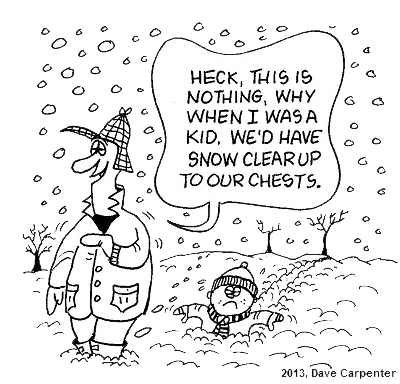
\includegraphics[width=8cm]{\texDirectory/template/images/windchill.png}
\end{figure}

\section*{Question 2}

Write a program \textit{Maximum.java} that takes three integer numbers as command-line arguments and prints their maximum, minimum and mean values.

\prepare{footer}

\end{document}
